% Source: Code/ML_overlay/ir_rgb_registration/paper/ml_overlay_report_materials/ir_rgb_registration_report/figures/fig_partial_overlap_examples.tex
\documentclass[tikz,border=10pt]{standalone}
\usepackage{tikz}

\definecolor{Garnet}{RGB}{115, 0, 10}
\definecolor{Atlantic}{RGB}{70, 106, 159}
\definecolor{Black30}{RGB}{199, 199, 199}
\definecolor{Black70}{RGB}{92, 92, 92}

\begin{document}
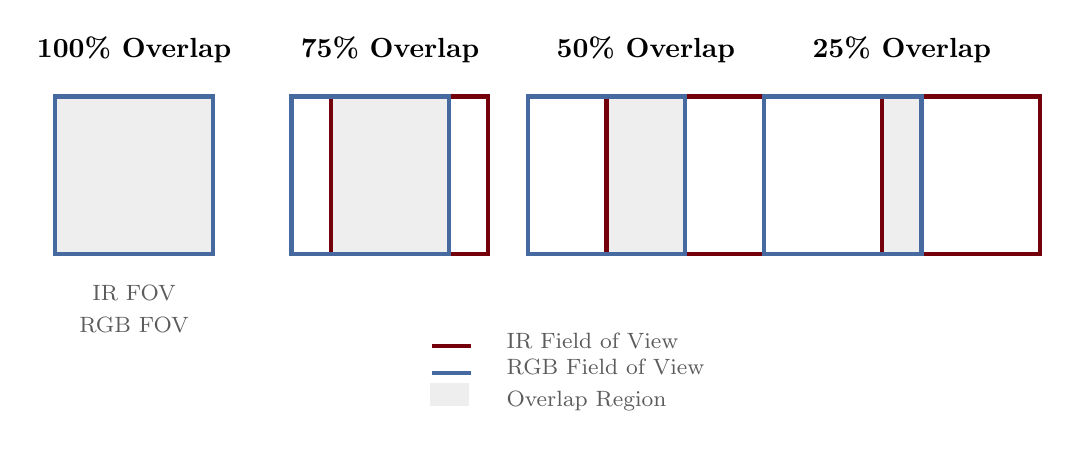
\begin{tikzpicture}

% Panel 1: 100% overlap
\begin{scope}[shift={(0,0)}]
    \fill[Black30, opacity=0.3] (0,0) rectangle (2,2);
    \draw[Garnet, line width=1.5pt] (0,0) rectangle (2,2);
    \draw[Atlantic, line width=1.5pt] (0,0) rectangle (2,2);
    \node[above, font=\bfseries] at (1,2.3) {100\% Overlap};
    \node[font=\footnotesize, Black70] at (1,-0.5) {IR FOV};
    \node[font=\footnotesize, Black70] at (1,-0.9) {RGB FOV};
\end{scope}

% Panel 2: 75% overlap
\begin{scope}[shift={(3.5,0)}]
    \fill[Black30, opacity=0.3] (0,0) rectangle (1.5,2);
    \draw[Garnet, line width=1.5pt] (0,0) rectangle (2,2);
    \draw[Atlantic, line width=1.5pt] (-0.5,0) rectangle (1.5,2);
    \node[above, font=\bfseries] at (0.75,2.3) {75\% Overlap};
\end{scope}

% Panel 3: 50% overlap
\begin{scope}[shift={(7,0)}]
    \fill[Black30, opacity=0.3] (0,0) rectangle (1,2);
    \draw[Garnet, line width=1.5pt] (0,0) rectangle (2,2);
    \draw[Atlantic, line width=1.5pt] (-1,0) rectangle (1,2);
    \node[above, font=\bfseries] at (0.5,2.3) {50\% Overlap};
\end{scope}

% Panel 4: 25% overlap
\begin{scope}[shift={(10.5,0)}]
    \fill[Black30, opacity=0.3] (0,0) rectangle (0.5,2);
    \draw[Garnet, line width=1.5pt] (0,0) rectangle (2,2);
    \draw[Atlantic, line width=1.5pt] (-1.5,0) rectangle (0.5,2);
    \node[above, font=\bfseries] at (0.25,2.3) {25\% Overlap};
\end{scope}

% Legend
\node[font=\footnotesize, Black70] at (6.5,-1.5) {
    \begin{tabular}{ll}
        \tikz\draw[Garnet, line width=1.5pt] (0,0) -- (0.5,0); & IR Field of View \\
        \tikz\draw[Atlantic, line width=1.5pt] (0,0) -- (0.5,0); & RGB Field of View \\
        \tikz\fill[Black30, opacity=0.3] (0,0) rectangle (0.5,0.3); & Overlap Region
    \end{tabular}
};

\end{tikzpicture}
\end{document}
